\documentclass[12pt,a4paper,notitlepage,english]{article}
\usepackage[utf8]{inputenc}
\usepackage{amsmath}
\usepackage{amsfonts}
\usepackage{longtable}
\usepackage{amssymb}
\usepackage{graphicx}
\usepackage[a4paper, left=.6in,right=.6in,top=.8in,bottom=.8in,]{geometry}
\usepackage{tabularx,ragged2e,booktabs,caption}
\usepackage{setspace}
\setstretch{1.5}
\usepackage{tabularx, booktabs}
\usepackage{dcolumn} 
  \newcolumntype{d}[1]{D{.}{.}{#1}}    
\newcolumntype{Y}{>{\centering\arraybackslash}X}
\usepackage[T1]{fontenc}
\usepackage{babel}
\usepackage{epigraph}
\usepackage{url}
\usepackage[round,sort]{natbib}
\newcommand{\source}[1]{\caption*{\footnotesize Source: {#1}} }
\usepackage{float}
\usepackage[section]{placeins}

\author{
  Guillaume Daudin\thanks{Université Paris-Dauphine, PSL Research University, LEDa, 75016 PARIS, FRANCE Université Paris-Dauphine, PSL Research University, IRD, LEDa, UMR 225, DIAL, 75016 PARIS, FRANCE Sciences Po, Observatoire Français des Conjonctures Économiques (OFCE), 75014 PARIS, FRANCE email: guillaume.daudin@dauphine.fr}
  \and
  Elisa Tirindelli\thanks{Trinity College Dublin, email: tirindee@tcd.ie}
}
\title{The futility of mercantilist wars \\ a case study of France between 1733 and 1820\thanks{The authors want to thanks Philip Hoffman for sharing data with them.}}
\date{}


\begin{document}

\maketitle






\begin{abstract}
Was Mercantilist warfare effective in its own terms, by crippling trade of defeated powers? Our paper explores the Anglo-French experience during the eighteenth century and contributes to understanding why that was not the case. Using new French data by product and by partner, we explore the general mechanisms relating trade and conflicts. We look into the product breakdown of trade to observe the difference in impact between goods. We find indeed a general negative impact on trade, but looking at the product breakdown, the effect is much stronger in the case of colonial products, whereas in the case of European products the impact was even positive. The post-war recovery of French trade is very quick. It took the Wars of the Revolution and the Napoleonic Wars and the Continental Blockade to actually cripple French trade.
\end{abstract}


\section{Introduction}

\epigraph{Savez-vous Messieurs ce qu’est une bataille navale ? On se rencontre, on se salue, on se canonne et la mer n’en reste pas moins salée.}{Maurepas, Navy Minister of Louis  \textsc{xv}, 1718-1748}



\maketitle


Is mercantilist warfare effective in its own terms, by crippling trade of defeated powers? Our paper explores the Anglo-French experience during the eighteenth century and contributes to understanding why that was not the case.
\cite{jefferson_letter_1823} famously noticed that European nations \textit{were nations of eternal war}. Indeed, from 1700 to 1825, 2 years out of 3 experienced conflict between major European powers \cite{roser_war_2016}. Rivalry between Great-Britain and France was central, so much as the period between 1688 to 1815 was called the « 2nd Hundred Years War » 1688-1815. War has many causes. Yet, especially after the death of Louis XIV, it cannot be denied that mercantile rivalry was an important motivation of Anglo-French wars (\cite{wallerstein_modern_1980, crouzet_guerre_2008}). Each nation was jealous of the other's commercial success. The British believed war was a good way to curtail them. The French partly agreed and were more wary of wars because they did not have much naval success. 
Here is the long list of wars between France and Britain after the death of Louis XIV: War of the Polish Succession (1733-1738) (little naval hostilities), War of the Austrian Succession (1740,–1748, where naval hostilities started in 1744), Seven Years' War (1756–1763), War of American independence (1775–1783, where French involvement started in 1778), French Revolutionary Wars (1792–1802) and Napoleonic Wars (1803–1815). Yet, all these wars were in vain before the 1790s, as French trade increased up to the British level throughout the eighteenth century (Figure \ref{FrBritTrade}).
Looking at peace-time trends (including land only wars), it is clear that French trade, despite big war shocks, was resilient and was not moved out of its pre-1744 trend (Figure \ref{FrPeaceTrade}). Things changed after 1815.
\begin{figure}
\caption{French, British trade and Anglo-French wars}
\centering
\includegraphics[scale=.6]{"Total silver trade FR GB".png}
\source{French trade up to 1821: \cite{daudin_toflit18_????}. French trade 1822-1840: \cite{federico_world_2016} / \cite{dedinger_exploring_2017},

England/British trade up to 1800: \cite{deane_british_1969}. UK trade from 1801 to 1840: \cite{federico_world_2016} / \cite{dedinger_exploring_2017},

Livre tournois silver value: \cite{de_wailly_memoire_1857} and \cite{hoffman_priceless_2000}; Pound sterling silver value: \cite{clark_england_1209-1914_2006} and \cite{jastram_silver_1981}}
\label{FrBritTrade}
\end{figure}

\begin{figure}
\caption{Peace time trends of total French trade}
\centering
\includegraphics[scale=.6]{"Peace-time trends of French trade".png}
\source{see Figure \ref{FrBritTrade} and author's computations}
\label{FrPeaceTrade}
\end{figure}
How come the pre-1792 wars did not have a lasting effect on French trade? This is important to understand the effect of wars in general, the geopolitical history of the eighteenth and nineteenth century and the globalization/deglobalization cycle from the 1490s to the 1840s.

\section{Literature}
There exists a vast literature focusing on the relationship between trade and war.
A first strand of this literature concentrates on the impact of trade on wars. Within this strand, two major perspectives have emerged: a liberal and a realist one. The first supports a vision of interdependence between trade and war, pointing out that trade promotes peace since it is a better method of expansion than wars. The second opposes this view by claiming that there is no impact of trade on wars, and if any, then it will be a positive impact, as countries will be pushed to move war to maintain trade supremacy.
The second strand of the literature, on the other hand, focuses on the impact of conflicts on trade. The works following this perspective are more homogeneous, and most authors agree to the disruptive effects on trade caused by wars. \cite{levy2004trading} analyse the impact of war on trade with adversary countries using seven dyads between 1870-1992, and they find that, although different across dyads, the general impact of conflict on trade is not particularly strong and mostly only temporary. \cite{blomberg2006much} analyse more specifically the effect of all kind of conflicts, distinguishing between internal and external, and find that peace has a large and positive impact on trade. \cite{anderton2001impact} look at the effect of wars on global trade, and find that when major world power are at war significant pre and post war effects are observed, whereas impact is much smaller for conflicts between minor powers. \cite{martin2008make} construct a theoretical model describing the likelihood of war and test it empirically; they find that likelihood of war is much smaller for countries involved in bilateral trade than for those involved in multilateral. Finally \cite{glick2010collateral} try to quantify the economic impact of the two world wars and claim that conflicts had negative effects on both belligerent and neutral countries with lags up to ten years. Altogether, the papers mentioned above do not always find coherent results, and such results were obtained from data from the last century only. The only exception is \cite{rahman2010fighting} who uses British trade data from eighteen century, but concentrates manly on the impact of naval conflicts on trade. The majority of scholars (apart from \cite{levy2004trading}) also finds long lasting effects of war; they claim commerce took several years before restoring its prewar level.\\
The effect of mercantilists wars on French trade does not fit this pattern. \cite{riley_seven_1986}, who concentrates on the case study of the Seven Years War, observes French trade series and he notices that there were no lags but on the contrary pre and post war loss compensation effects. This widely recognized fact about the effect of eighteenth century wars on French trade has led historians to research extensively the strategies of French merchants to cope with war. Neutral carriers were somewhat protected from British predation on the sea. When necessary, French merchants could even hide their cargo ownership behind a neutral partner. Or they could move to neutral countries and operate from there (\cite{marzagalli_was_2016}). Historians have even reflected that war periods might have been necessary to the functioning of the \textit{Éxclusif Colonial}, i.e. the theoretical monopoly of French merchants on French colonial trade (\cite{lespagnol_mondialisation_1997, morineau_vraie_1997, marzagalli_was_2016}). The argument rests on the large peace time trade imbalances between France and its Northern European clients for colonial goods that could have been balanced by large service income of Northern European merchants during war time as they, as neutrals, provided shipping and various trade services to the French empire. The quality of the available balance of payment data is not good enough to test that hypothesis.\\
The aim of this paper is to extend \cite{riley_seven_1986}’s work by analysing the available French data in the eighteenth century. So far the literature has analysed the impact on trade of twentieth century wars and generalized the results. We believe that the effect of wars in twentieth century is different from that of other wars throughout history, and related data offer only a partial point of view. Thus, we are convinced that analysing less recent data is crucial to understand the general mechanisms relating trade and conflicts. We focus on the difference in impact depending on kind of war and on war status. We distinguish three possible ways of grouping conflicts, the first encompasses all wars in general, the second distinguishes between Mercantilist wars and Napoleonic and Revolutionary wars and the third differentiates between wars and the Continental Blockade. We also look into the product and sector breakdown of trade to observe the difference in impact between main goods and sectors. We find indeed a general negative impact on trade with foes, however the impact on trade with neutral countries is not as well defined. In fact, when testing for the first two groups of conflicts mentioned, commercial relations with neutral countries are not damaged. It is only when distinguishing between wars and Continental Blockade that we observe that trade is actually disrupted also towards/from neutral countries. This leads us to think that wars were not the main source of disruption for trade, before at least twentieth century, because during wars, neutral countries could still manage to trade relatively freely and most likely take over the trade from belligerent countries. It was only during the Continental Blockade, when commerce with neutral countries was also restricted, that French trade experienced a decline. This avails the hypothesis of the role of neutral countries in modern trade and its importance for its success. 

\section{Dataset}
\subsection{Origin of the data}
For conducting our analysis we use data from the archives of the French \textit{Bureau de la Balance du Commerce}. This institution was created in 1713, after the Treaty of Utrecht, which followed the Spanish succession war. In this circumstances, the French were positively impressed by the detailed knowledge shown by the British on their trade flows and they also decided to create an institution which would keep track of exports and imports from and to France. Before this, there were already local institutions keeping track of goods going in and out of harbour cities (only in quantity terms) but starting 1716 they started sending their records to the \textit{Bureau}. The \textit{Bureau} would then compute aggregate yearly figures for each \textit{direction} (port) and then send them back to the local chamber of commerce, so that they could add the values. Unfortunately those documents did not survive till our days; we still have some records from local sources but they are quite incomplete. On the other hand, another kind of document survived, which reports the total value of trade for each destination for each year, so at least we have reliable figures on aggregate values. Starting from 1750 the \textit{Object Général} was introduced, which was more complete, and was recording each product from and to each destination for all ports. The \textit{Objet Général} survived in its entirety and this is what we have used for my estimations. For the period preceding 1733, we have estimated the data basing on local sources, as explained in section 3. \\
\subsection{Figures}
For the period between 1733 and 1820, this dataset accounts for 146,963 observations, with incomplete data between 1761 and 1767 and missing data between 1782 and 1787, in 1789 and in 1797. There are overall 82 different destinations recorded, but each one of them is not present every year. Rather than single countries they are groups of countries and most destinations get broken down into smaller destinations in later periods or even disappeared to be replaced by other smaller entities. To bypass this problem we used country grouping. Eleven different groups could be created and each of them comprises all the evolution of one destination, so that we can have observations for each group for each year. The groups we are considering are: Germany, England, Flanders and Habsburg Monarchy, Italy, Portugal, Spain, Switzerland, Colonies, Dutch Republic, India, Levant, North. The same issue arises with products, there are 4,695 different products recorded, which we have re-classified in 40 different categories or 20 sectors. For the breakdown by product and sectors though, we are mainly focusing on coffee, sugar, wine and eau-de-vie, which represent the main share of Colonial and European products exported. \\
Values in the dataset are always expressed in \textit{livres turnois}, but we will convert them in grams of fine silver to have a comparable estimate year to year. The value of the \textit{livre} has been constant at 4.505 grams of fine silver all throughout the period in consideration.

\subsection{Limitation and Missing data}
As mentioned above, for the whole period preceding 1749, the only available data we have from the French source is either the yearly aggregate figures by destination, or the incomplete local sources, which on the other hand contains information on each product. For this reason, in order to perform the comparison between the two datasets and the subsequent analysis, it will be necessary to estimate the full value of exports from the available data. In order to do this, we run the following regression:
\begin{center}
$\ln(product_{i,j,k,t})=\beta_0 + \beta_1year_t+\beta_3direction_k$
\end{center}
where the dependent variable products stands for the value of exports of one product, for each port reported in the local source and for each year. Year is a set of year dummies and direction is also a set of dummies that indicates in which port the data were recorded (direction also includes "France", meaning all ports). This model aims at predicting the export value of single products per year basing on the yearly changes in export and on the export composition by source, with the assumption that the composition is constant overtime. We run the model on the whole available years but we only do so for coffee, sugar, wine, eau-de-vie and an aggregate category of all other goods (other). In addition, to avoid the problem of log of zero trade flows, we have substituted them with 0.001, so that observations would not drop but the zero flows in the estimation could be taken into account as a value really close to zero. Finally, we also added weights on value, as to give more importance to flows higher in value. The results are pretty satisfactory, in fact the pattern of estimated and actual value are very similar. 

\section{Historical summary}
\subsection{War of Polish Succession}
The war of Polish succession took place between 1733 and 1738. It started with the death of the king of Poland August II who died heirless and soon become a conflict at European level. France, Prussia and Spain were trying to limit the desire of expansion of the Habsburg monarchy, which was aiming at extend its power over Poland. The lack of support by England however, concluded the war in 1738, with the recognition of August III as king of Poland. The belligerent countries were France, Spain and Italy on the one side and the Habsburg Monarchy on the other. 

\subsection{War of Austrian Succession}
The war of Austrian succession was a European conflict that burst in 1740 over the eligibility to succession to the crown of Maria Theresa of Austria, as the heir of the Habsburg Monarchy after the death of her father. It started out as a European conflict but after 1744 it involved also the colonies. Belligerent countries were France, Spain, Prussia and Italy on one side and England, Habsburg monarchy and the Dutch Republic on the other. 

\subsection{Seven Years Wars}
The Seven year war was a major conflict, which took place between 1756 and 1763. It is consider the first real world conflict and European powers were fighting over possession of colonies. Belligerents countries were: England, Prussia and Portugal on one side and France, Spain, Habsburg monarchy, and Dutch Republic on the other. 

\subsection{American Revolutionary War}
The American Revolutionary War took place between 1778 and 1782. In this case the field of battle was not Europe anymore, but directly the Colonies. British North American colonies were rebelling against Britain control over their trade and were fighting for independence. Belligerent countries were England on the one side and France, Spain and British Colonies on the other (later United States). During this war the First League of Armed Neutrality was signed between Russia, Sweden and Denmark. Spain accepted this agreement however Britain demurred. When Dutch Republic was about to join this league, Britain found out before the treaty was signed and captured a Dutch ships, thus forcing the Dutch to enter war against them. Starting 1781 therefore, the Dutch Republic also became a belligerent country, allied to France. 

\subsection{French Revolutionary Wars}
The French Revolutionary Wars took place between 1792 and 1802. It was a conflict that had started as a consequence of French Revolution, in 1789, with the hope of spreading the revolutionary ideas around Europe. During this war, France and Spain were fighting against most of the rest of Europe, in particular Great Britain and the Habsburg Monarchy. France experienced an unexpected success in continental Europe, because of the raise in power of general Napoleon Bonaparte, however was on the other hand heavily defeated by the Royal Navy, thus loosing supremacy over the Mediterranean and also its colonies. This conflict was ended by the Treaty of Amiens in 1802, which started the only year of peace in Europe between 1792 and 1815.

\subsection{Napoleonic Wars}
The Napoleonic wars were a series of conflict between the French Empire of Napoleon I and  other countries, primarily led by the British, which took place in the years 1803 to 1815. Its consequences were the final defeat of Napoleon, and the First French Empire, and the rise of the British Empire as the world's premier power. On the other hand, this conflict contributed to spread all over Europe the nationalist and liberal ideas that were born during the French Revolution, despite the restoration of the monarchy in France and the decay of the Revolutionary principles. 

\subsection{Continental Blockade}
The Continental Blockade (1806 to 1914) was the foreign policy adopted by Napoleon against the United Kingdom during the Napoleonic Wars. It consisted in a large-scale embargo against British trade where all commercial connections of Britain to the Continent were supposed to be interrupted. It was only stopped in 1814, with Napoleon's abdication. 

\section{Empirical Analysis}
As mentioned above, the period in analysis was a period of "eternal war". The aim of this study is to uncover what were the effects of this long-lasting war status and to identify the drivers of the massive loss in trade at the end of century. The unique database we are using allows us to do so in more details than it has been done so far. In fact, we are not only doing it for aggregate trade for all countries but also distinguishing between neutral and foes and looking at a breakdown by products and sectors. \\
The first distinction is because we aim at uncovering the weight of neutral trade on global commerce in the eighteenth century. The role of neutral has long been discussed and we aim to contribute to this debate. The second is to observe variations in impact across products and sectors. Products were traded from and to very different places, and it is legitimate to believe they might have been impacted differently. For this reason we want to observe the effect of conflicts on specific products as well. \\
This latter task, however, was not an easy one. The number of reported products is quite high and mostly they do not appear repeatedly (They either have different names or they are grouped together with different products). For this reason we have chosen to use only the two main European products (Wine and Eau-de-vie) and the two main colonial products (Coffee and Sugar), which also represent the main share of French trade at the time, in value terms. We have aggregated all the other products in one single category which we refer to as "Other". As for the sectoral study, things were a bit easier, as we were able to classify all the products using the SITC classification. \\
Instead of looking at each war, one by one, we have created the following two types of war: Mercantilist Wars (between 1744 and 1808) and Blockade Wars (from 1808 to 1820). The former differs from the latter in that the political settings in second half of the eighteenth century were altered as a consequence of the French Revolution. Therefore, we decided to make a distinction between wars before 1808, which were rather driven by economic interest, and the Continental Blockade, which, on the other hand, had more of a political goal. Also, in that same period, a technological change took place, that allowed the British Navy to keep ships out of their ports more efficiently. This dramatically reduced smuggling and allowed British to impede unwanted trade more efficiently. 
Finally, we are more interested in the impact of wars in general, rather than each single war of the eighteenth century. 
In the robustness section of this paper we also use two other possible classifications. We do so both for imports and exports, running the following specifications: 
\begin{multline}\label{eq:1}
Flow_{t}=\exp\{\beta_0+\beta_1Status_jWar_k + \beta_2WarYearStatus_jWar_k+\beta_3Country_l +\beta_4YearCountry_l\}
\end{multline}
Where $Status_j$ is a dummy which indicates either foe or neutral, $War_k$ is another dummy which takes value 1 during the years of war, or is an indicator for which kind of war is taking place, $Year$ is the time trend and $Country_l$ and $YearCountry_l$ are respectively country fixed effects and year time trend. This first specification provides information on the effects of war, or groups of war, depending on the situation of the country at stake (neutral of foes). 
\begin{multline}\label{eq:2}
Flow_{t}=\exp\{\beta_0+\beta_1Status_jWar_k + \beta_2WarYearStatus_jWar_k+\beta_3Country_lProduct_i +\\ +\beta_4YearCountry_lProduct_i\}
\end{multline}
Equation \ref{eq:2} differs from equation \ref{eq:1} in that we have run on the database disaggregated by product and we have used country-product fixed effects and country-product time trend instead.  
\begin{multline}\label{eq:3}
Flow_{t}=\exp\{\beta_0+\beta_1Status_jWar_k + \beta_2Country_lProduct_i+\beta_3YearCountry_lProduct_i\}
\end{multline}
Specification \ref{eq:3} allows us to look at effects of each group of war on the trade with allies and foes, by using product fixed effects and country-product time trend.
\begin{multline}\label{eq:4}
Flow_{t}=\exp\{\beta_0+\beta_1Product_iWar_k + \beta_2WarYearProduct_iWar_k+\beta_3Product_i +\\ +\beta_4YearProduct_i\}
\end{multline}
In equation \ref{eq:4} we are testing again the effects of kind of wars on products but by using product fixed effects and time trend, as opposed to country-product fixed effects and trends. 
\begin{multline}\label{eq:5}
Flow_{t}=\exp\{\beta_0+\beta_1Product_iWar_k + \beta_2WarYearProduct_iWar_k+\beta_3Country_lProduct_i +\\ +\beta_4YearCountry_lProduct_i\}
\end{multline}
In this fifth specification $WarYearProduct$ is the time trend computed only over the war years and $War_k$ is interacted with $Product_i$, so we can observe the effect of the different kind of conflicts on the specific products. 
\begin{multline}\label{eq:6}
Flow_{t}=\exp\{\beta_0+\beta_1Product_iWar_k + \beta_2Product_iCountry_l+\beta_3YearCountry_lProduct_i\}
\end{multline}
Finally, equation \ref{eq:6} provides an insight for the effects of groups of wars on specific products. \\
We start by using exports as explained variable and the five goods as \textit{products} (coffee, sugar, wine, eau-de-vie and others), in all the above mentioned six specifications. Later we will repeat the analysis using imports and sectors. 
Table \ref{table:export_class_war} reports the result of the first case where we have used a dummy just for peace or war, with no distinction on the kind of conflict.
\begin{table}
\begin{center}
\caption {Exports, Mercantilist Wars and Continental Blockade} 
\label{table:export_class_block}
\renewcommand{\arraystretch}{0.6}
{
\def\sym$\times$1{\ifmmode^{$\times$1}\else\(^{$\times$1}\)\fi}
\begin{tabular}{l*{6}{c}}
\hline\hline\\
                    &\multicolumn{1}{c}{(1)}&\multicolumn{1}{c}{(2)}&\multicolumn{1}{c}{(3)}&\multicolumn{1}{c}{(4)}&\multicolumn{1}{c}{(5)}&\multicolumn{1}{c}{(6)}\\
\hline\\
Allies$\times$Blockade&       0.227         &       0.195         &     -0.0252         &                     &                     &                     \\
                    &      (1.27)         &      (1.45)         &     (-0.24)         &                     &                     &                     \\
[1em]
Allies$\times$Mercantilist&      -0.130         &      -0.126         &     -0.0444         &                     &                     &                     \\
                    &     (-1.51)         &     (-1.55)         &     (-0.59)         &                     &                     &                     \\
[1em]
Foes$\times$Blockade&      -0.675** &      -0.676** &     -0.0201         &                     &                     &                     \\
                    &     (-2.71)         &     (-3.06)         &     (-0.17)         &                     &                     &                     \\
[1em]
Foes$\times$Mercantilist&      -0.463         &      -0.443         &      -0.560*  &                     &                     &                     \\
                    &     (-1.18)         &     (-1.27)         &     (-2.35)         &                     &                     &                     \\
[1em]
Neutral$\times$Blockade&      -1.403***&      -1.377** &      -0.586** &                     &                     &                     \\
                    &     (-3.35)         &     (-3.08)         &     (-2.99)         &                     &                     &                     \\
[1em]
Neutral$\times$Mercantilist&     -0.0809         &     -0.0265         &      -0.164*  &                     &                     &                     \\
                    &     (-0.66)         &     (-0.25)         &     (-2.02)         &                     &                     &                     \\
[1em]
Coffee$\times$Blockade&                     &                     &                     &      -2.966** &      -2.970***&      -2.891***\\
                    &                     &                     &                     &     (-3.25)         &     (-3.89)         &     (-4.93)         \\
[1em]
Coffee$\times$Mercantilist&                     &                     &                     &      -0.314         &      -0.305         &      -0.388         \\
                    &                     &                     &                     &     (-0.93)         &     (-1.20)         &     (-1.14)         \\
[1em]
Eau de vie$\times$Blockade&                     &                     &                     &       0.398         &       26.42         &       28.80         \\
                    &                     &                     &                     &      (1.43)         &      (0.94)         &      (1.03)         \\
[1em]
Eau de vie$\times$Mercantilist&                     &                     &                     &      -0.367         &       25.90         &       28.61         \\
                    &                     &                     &                     &     (-1.08)         &      (0.92)         &      (1.02)         \\
[1em]
Other$\times$Blockade&                     &                     &                     &     -0.0599         &      -35.28         &      -35.98         \\
                    &                     &                     &                     &     (-0.79)         &     (-1.05)         &     (-1.07)         \\
[1em]
Other$\times$Mercantilist&                     &                     &                     &      -0.177         &      -35.37         &      -36.12         \\
                    &                     &                     &                     &     (-1.49)         &     (-1.05)         &     (-1.07)         \\
[1em]
Sugar$\times$Blockade&                     &                     &                     &      -3.813***&       122.7** &       126.3** \\
                    &                     &                     &                     &     (-4.07)         &      (2.95)         &      (2.97)         \\
[1em]
Sugar$\times$Mercantilist&                     &                     &                     &      -0.151         &       126.5** &       130.0** \\
                    &                     &                     &                     &     (-0.51)         &      (3.05)         &      (3.06)         \\
[1em]
Wine$\times$Blockade&                     &                     &                     &      -0.189         &       22.18         &       21.40         \\
                    &                     &                     &                     &     (-0.91)         &      (0.81)         &      (0.78)         \\
[1em]
Wine$\times$Mercantilist&                     &                     &                     &      -0.241         &       22.26         &       21.30         \\
                    &                     &                     &                     &     (-1.32)         &      (0.81)         &      (0.78)         \\
[1em]
Constant            &      -20.17***&      -63.73***&      -64.62***&      -0.320         &      -75.42***&      -75.36***\\
                    &     (-4.29)         &     (-3.55)         &     (-3.64)         &     (-0.03)         &     (-3.90)         &     (-3.88)         \\
\hline\\
Observations        &        1010         &        5050         &        5050         &         445         &        5050         &        5050         \\
\hline\hline
\multicolumn{7}{l}{\footnotesize \textit{t} statistics in parentheses}\\
\multicolumn{7}{l}{\footnotesize * \(p<0.05\), ** \(p<0.01\), *** \(p<0.001\)}\\
\end{tabular}
}

\end{center}
\end{table}
\begin{table}
\begin{center}
\caption {Imports, Mercantilist Wars and Continental Blockade} 
\label{table:import_class_block}
\renewcommand{\arraystretch}{0.6}
{
\def\sym$\times$1{\ifmmode^{$\times$1}\else\(^{$\times$1}\)\fi}
\begin{tabular}{l*{6}{c}}
\hline\hline
                    &\multicolumn{1}{c}{(1)}&\multicolumn{1}{c}{(2)}&\multicolumn{1}{c}{(3)}&\multicolumn{1}{c}{(4)}&\multicolumn{1}{c}{(5)}&\multicolumn{1}{c}{(6)}\\
\hline
Allies$\times$Blockade&     -0.0395         &      0.0222         &      -0.265*  &                     &                     &                     \\
                    &     (-0.18)         &      (0.18)         &     (-2.57)         &                     &                     &                     \\
[1em]
Allies$\times$Mercantilist&      -0.183         &      -0.154         &      -0.135*  &                     &                     &                     \\
                    &     (-1.55)         &     (-1.81)         &     (-2.19)         &                     &                     &                     \\
[1em]
Foes$\times$Blockade&      -0.561         &      -0.379         &      -0.173*  &                     &                     &                     \\
                    &     (-1.86)         &     (-1.89)         &     (-1.96)         &                     &                     &                     \\
[1em]
Foes$\times$Mercantilist&      -0.497         &      -0.478         &      -0.642***&                     &                     &                     \\
                    &     (-1.55)         &     (-1.75)         &     (-3.42)         &                     &                     &                     \\
[1em]
Neutral$\times$Blockade&      -1.146***&      -1.115***&      -0.737***&                     &                     &                     \\
                    &     (-3.42)         &     (-3.90)         &     (-5.36)         &                     &                     &                     \\
[1em]
Neutral$\times$Mercantilist&     -0.0261         &      0.0177         &     -0.0625         &                     &                     &                     \\
                    &     (-0.26)         &      (0.21)         &     (-1.01)         &                     &                     &                     \\
[1em]
Coffee$\times$Blockade&                     &                     &                     &      -2.135***&      -2.007***&      -2.061***\\
                    &                     &                     &                     &     (-5.93)         &     (-4.19)         &     (-6.12)         \\
[1em]
Coffee$\times$Mercantilist&                     &                     &                     &      -0.597*  &      -0.554*  &      -0.498*  \\
                    &                     &                     &                     &     (-2.09)         &     (-2.13)         &     (-2.09)         \\
[1em]
Eau de vie$\times$Blockade&                     &                     &                     &       0.183         &       41.31         &       43.52         \\
                    &                     &                     &                     &      (0.70)         &      (1.61)         &      (1.72)         \\
[1em]
Eau de vie$\times$Mercantilist&                     &                     &                     &      -0.350         &       40.89         &       43.50         \\
                    &                     &                     &                     &     (-1.17)         &      (1.60)         &      (1.73)         \\
[1em]
Other$\times$Blockade&                     &                     &                     &      -0.150*  &       19.45         &       19.71         \\
                    &                     &                     &                     &     (-2.18)         &      (1.04)         &      (1.06)         \\
[1em]
Other$\times$Mercantilist&                     &                     &                     &      -0.101         &       19.47         &       19.74         \\
                    &                     &                     &                     &     (-1.19)         &      (1.05)         &      (1.06)         \\
[1em]
Sugar$\times$Blockade&                     &                     &                     &      -1.371         &       68.46** &       68.73** \\
                    &                     &                     &                     &     (-1.54)         &      (2.76)         &      (2.77)         \\
[1em]
Sugar$\times$Mercantilist&                     &                     &                     &      -0.329         &       69.37** &       69.84** \\
                    &                     &                     &                     &     (-1.19)         &      (2.80)         &      (2.82)         \\
[1em]
Wine$\times$Blockade&                     &                     &                     &      -0.210         &       39.24         &       38.63         \\
                    &                     &                     &                     &     (-1.03)         &      (1.53)         &      (1.50)         \\
[1em]
Wine$\times$Mercantilist&                     &                     &                     &      -0.236         &       39.29         &       38.54         \\
                    &                     &                     &                     &     (-1.33)         &      (1.53)         &      (1.50)         \\
[1em]
Constant            &      -27.31***&      -84.87***&      -85.02***&      -17.63*  &      -94.32***&      -94.32***\\
                    &     (-5.78)         &     (-7.84)         &     (-7.90)         &     (-2.28)         &     (-7.50)         &     (-7.53)         \\
\hline
Observations        &        1010         &        9792         &        9792         &         445         &        9792         &        9792         \\
\hline\hline
\multicolumn{7}{l}{\footnotesize \textit{t} statistics in parentheses}\\
\multicolumn{7}{l}{\footnotesize * \(p<0.05\), ** \(p<0.01\), *** \(p<0.001\)}\\
\end{tabular}
}

\end{center}
\end{table}
The six regressions in table \ref{table:export_class_block} report the results. For this set of analysis we have split the conflicts again in two groups, but this time distinguishing between any war (1717-1787) and Continental Blockade (from 1808). In this setting we notice a difference with respect to the pattern seen before. Adversaries see a decrease in trade only according to specification \ref{eq:1} and \ref{eq:2} but not to specification \ref{eq:3}, however, neutral during the Blockade years, experience a very substantial decrease in trade. This would suggest that, whereas wartime was mostly damaging for trade towards enemies, the continental Blockade period, during which overall French trade lost to British, had damaged neutral countries, rather than Britain, which was the original target. It is quite likely, therefore, that before the Blockade had taken place, war did not represent such a danger for merchants, who were able to continue their trade through other channels, i.e. "neutral cargo" policy. On the other had, during Continental Blockade years, which were meant to damage British trade, regulation on neutral cargo had become much stricter, and this is where we observe a collapse in trade with neutral countries and a massive decrease in overall trade. As a consequence, we are prone to avail \cite{riley_seven_1986}'s theory on the small effects of wars on commerce, at least until the twentieth century, thanks to the ability of merchants to exploit neutral ships and workaround of wartime restrictions.\\
We repeat now all the three different analysis above on imports and we report them in tables \ref{table:import_class_war} to \ref{table:import_class_block}. From table \ref{table:import_class_war} we observe a very similar pattern with respect to the previous analysis. Wars in general are disruptive for trade towards foes, however there is no coherent evidence that neutral and allies were strongly affected at all. By looking at table \ref{table:import_class_merc} we observe, again, that imports from foes were strongly affected by Revolutionary and Napoleonic conflicts. Differently from before, there is a negative effect for allies, which was not the case for exports, and also a mild but significant impact for neutral countries during Mercantilist wars. Product-wise the situation is again similar, as we observe strong decrease in import of sugar but again an increase in import of eau-de-vie. As for table \ref{table:import_class_block}, once more it is evident the massive effect of the blockade on neutral trade. Not only exports but also imports from neutral countries were seriously damaged by the Blockade, way less so than imports from enemies. This goes once more in the direction of explaining the fall in trade of aggregate trade in the first half of the nineteenth century in France. \\
\iffalse
The results of this estimate also reflect the evolution of the role of neutral trade throughout the century and a half of wars. Initially, the only enemy were foes, whereas neutral countries were allowed to continue their trade with all other partners, despite an ongoing conflict. This rule, however, had induced belligerent countries to exploit neutral ships for trading their own merchandises (Carrière 1973). For this reason, in 1756, during Seven Years War, the British decided to put an end to this practice and produced the \textit{Doctrine of Continuous Voyage}, which was forbidding neutrals, in time of war, to enjoy a trade from which they were barred in time of peace. This prohibition was allowing the British to seize neutral shipping and had a considerable impact on French trade, which was heavily relying on Dutch ships to transport colonial goods. It also created great discontent on the side of neutral countries, which, however, were not able to express efficiently their disappointment until 1780, when a League of Armed Neutrality was created. The latter allowed neutral countries to keep trading more or less peacefully during the subsequent conflict, the War of American Revolution.
This experiment however did not have much success in its purposes and was finally put to an end in 1783 with the treaty of Paris, when Catherina of Russia renamed it the \textit{Armed Nullity} (Griffiths, 1971). 
\fi


%The figures below give a more visual picture of the trend of the different products. As for wine and eau-de-vie, war do not seem to have a great impact on their trend. As for coffee and sugar, on the other hand, wars seem to be diminishing trade, however, given the big fluctuations all throughout, we cannot for sure distinguish between the effects of conflicts and the very variable pattern of trade. 
%\begin{figure}[H]
%\begin{center}
%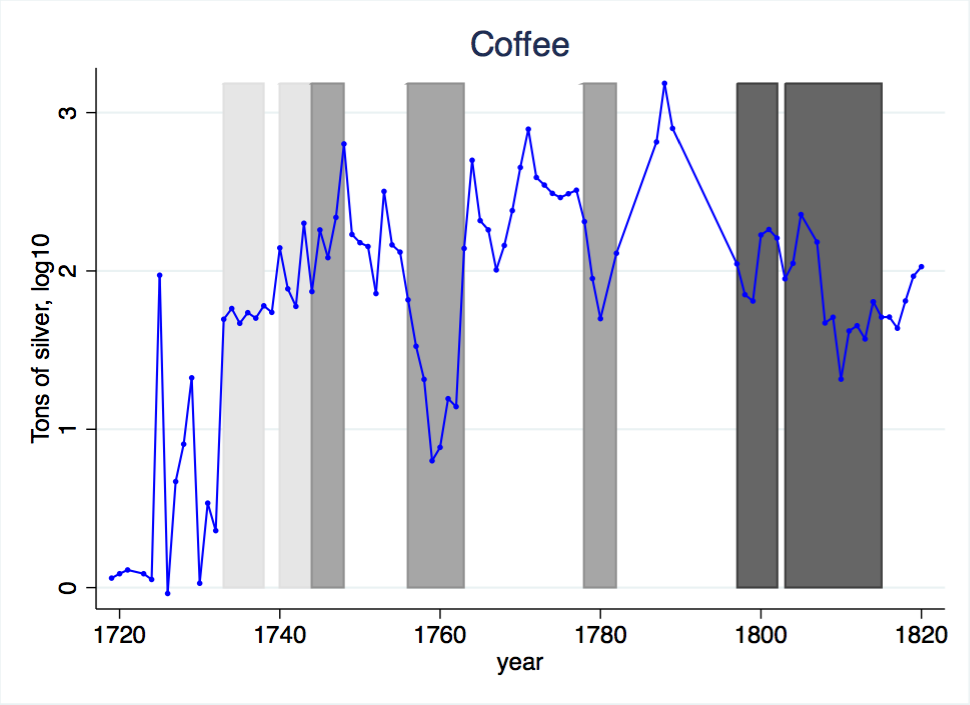
\includegraphics[scale=.25]{class1_trend}
%\hfil 
%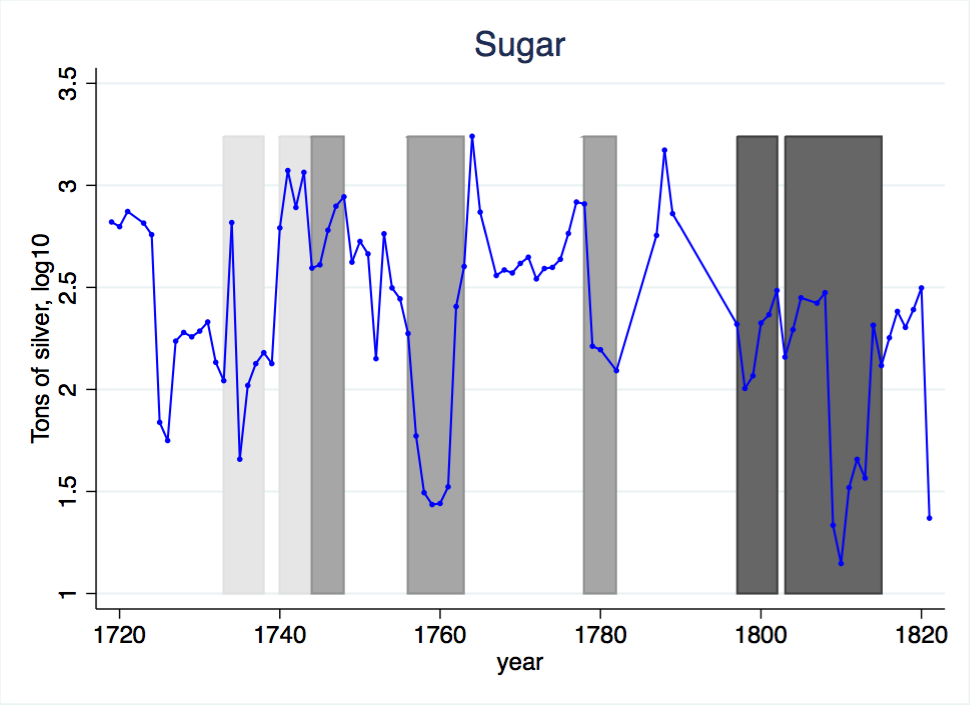
\includegraphics[scale=.25]{class3_trend}
%\vspace*{.7em}
%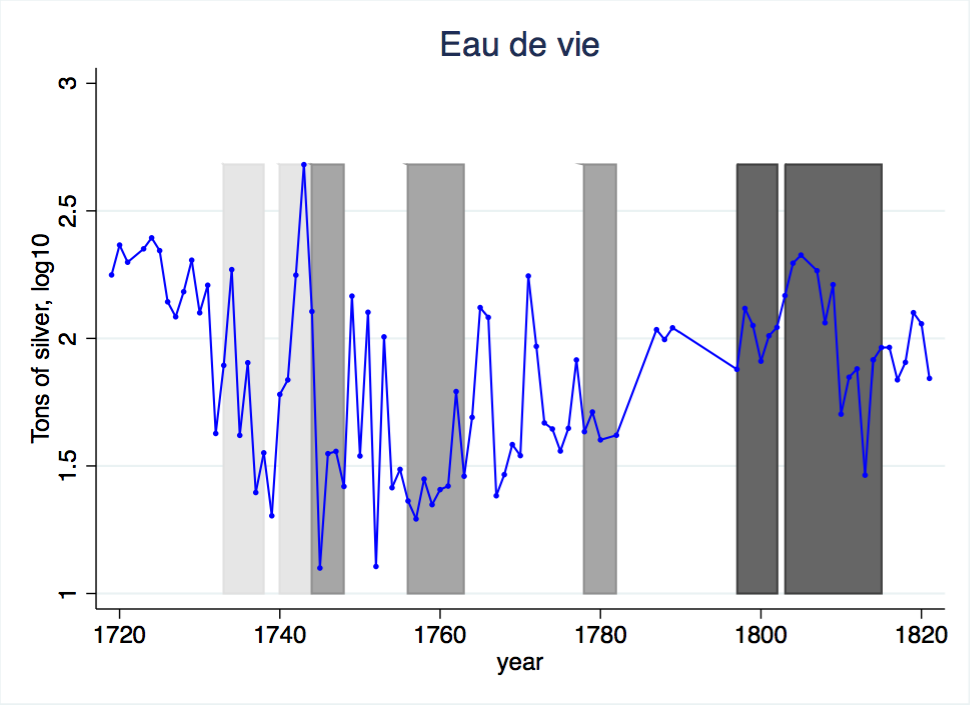
\includegraphics[scale=.25]{class2_trend}
%\hfil 
%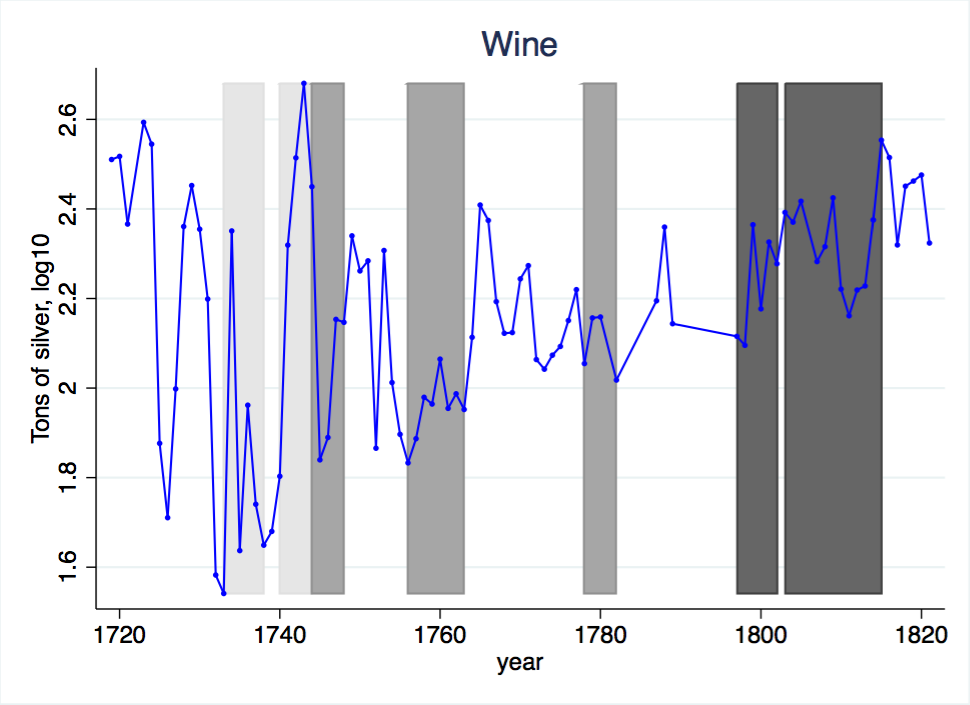
\includegraphics[scale=.25]{class4_trend}
%\end{center}
%\end{figure}

\iffalse
\subsection{War lags}
In line with this reasoning, we turned next to analyse and compare war lags in the Hamburg case and general case. we run two regressions with and without product differentiation and for all wars together and a dummy for each war: 
\begin{multline}
\ln(exports_{i,t})=\beta_0+\beta_1country_i+\beta_2country_iyear+\beta_3adversaries_i+\beta_4neutral_i+\\+\beta_5adversary_ilag+\beta_6neutral_ilag+\beta_8allies_ilag
\end{multline}
\begin{multline}
\ln(exports_{i,t})=\beta_0+\beta_1country_i+\beta_2country_iyear+\beta_3product_{i,j}+\beta_4product_jyear+\\+\beta_5product_jadversary+ \beta_6product_jneutral+\beta_7product_jadversary_ilag+\beta_8neutral_ilag+\beta_9allies_ilag
\end{multline}

Results are quite in line with those seen in the Hamburg series. There is no post war negative coefficient, but on the contrary, trade increases by 40\% and 47\% in the first and second year after the war. Starting from the third year this effect decreases and coefficients are still positive but smaller. \\
Product-wise there is evidence of positive post war effects for all the products but in particular European products increase stably for the first four years after the war. War by war, we notice an interesting pattern after Seven Years War; exports of European goods increases as for the general case, but here we see that trade of sugar as well expands right after the war (+62\%). This is quite an interesting result given that sugar was, with coffee, the product which suffered the most during this conflict. 
In sum, we can say that, as for the case of Hamburg, there is no clear evidence of war lags, for sure not 10 years lag as claimed by Glick and Taylor (2005). Trade was extremely adaptive to conflicts in eighteenth century and neutral countries did not seem to suffer strong consequences.
we have also run the regression checking for pre war effects. Results are positive but very small in size for the general case, except for the case of allies countries, which has larger and more significant coefficients. The war-by-war case (considered all in one regression) is also not very meaningful; coefficients for Seven Years War are negative whereas those for American Revolutionary War are positive. In terms of difference between products, the results are again not very interesting. There is no stable pattern for pre war effect, except for coffee, which always shows an increase for all the four years preceding the war. However this might be just due to the increasing trend shown by coffee, disregarding the effects of wars.
Overall, for neutral countries the compensation effect is more likely as a post war phenomenon rather than a pre war one, again as noted for the case of Hamburg. 
\fi

\section{Robustness}
We have re-run our analysis using two other possible grouping of wars. First considering all wars together (i.e. one dummy that takes value 1 whenever there is an ongoing conflict) and then by  Mercantilist wars (Polish and Austrian Succession, Seven Years War, American Revolutionary war) and Napoleonic and Revolutionary wars. 
Table \ref{table:export_class_war} reports the result of the first case where we have used a dummy just for peace or war, with no distinction on the kind of conflict.
\begin{table}
\begin{center}
\caption {Exports, for all wars together} 
\label{table:export_class_war}
\renewcommand{\arraystretch}{0.6}
{
\def\sym$\times$1{\ifmmode^{$\times$1}\else\(^{$\times$1}\)\fi}
\begin{tabular}{l*{6}{c}}
\hline\hline
                    &\multicolumn{1}{c}{(1)}&\multicolumn{1}{c}{(2)}&\multicolumn{1}{c}{(3)}&\multicolumn{1}{c}{(4)}&\multicolumn{1}{c}{(5)}&\multicolumn{1}{c}{(6)}\\
\hline
Allies$\times$War&     -0.0800         &     -0.0691         &     -0.0619         &                     &                     &                     \\
                    &     (-0.92)         &     (-0.85)         &     (-0.91)         &                     &                     &                     \\
[1em]
Foes$\times$War&      -0.768*  &      -0.735*  &      -0.319*  &                     &                     &                     \\
                    &     (-2.20)         &     (-2.53)         &     (-2.27)         &                     &                     &                     \\
[1em]
Neutral$\times$War&      -0.114         &     -0.0480         &      -0.208** &                     &                     &                     \\
                    &     (-0.92)         &     (-0.46)         &     (-2.64)         &                     &                     &                     \\
[1em]
Coffee$\times$War&                     &                     &                     &      -0.116         &      -0.106         &      -0.594         \\
                    &                     &                     &                     &     (-0.31)         &     (-0.38)         &     (-1.57)         \\
[1em]
Eau-de-vie$\times$War&                     &                     &                     &      -0.396         &       21.29         &       16.41         \\
                    &                     &                     &                     &     (-1.35)         &      (0.79)         &      (0.62)         \\
[1em]
Other$\times$War&                     &                     &                     &      -0.218*  &      -40.06         &      -46.26         \\
                    &                     &                     &                     &     (-1.98)         &     (-1.22)         &     (-1.44)         \\
[1em]
Sugar$\times$War&                     &                     &                     &     -0.0190         &       132.0***&       147.4***\\
                    &                     &                     &                     &     (-0.06)         &      (3.30)         &      (3.61)         \\
[1em]
Wine$\times$War&                     &                     &                     &      -0.357*  &       16.57         &       10.72         \\
                    &                     &                     &                     &     (-2.15)         &      (0.62)         &      (0.41)         \\
[1em]
Constant            &      -20.79***&      -64.20***&      -65.73***&       1.256         &      -71.81***&      -67.07***\\
                    &     (-4.28)         &     (-3.62)         &     (-3.68)         &      (0.12)         &     (-3.93)         &     (-3.85)         \\
\hline
Observations        &        1010         &        5050         &        5050         &         445         &        5050         &        5050         \\
\hline\hline
\multicolumn{7}{l}{\footnotesize \textit{t} statistics in parentheses}\\
\multicolumn{7}{l}{\footnotesize * \(p<0.05\), ** \(p<0.01\), *** \(p<0.001\)}\\
\end{tabular}
}

\end{center}
\end{table}
From table \ref{table:export_class_war}, where we only consider wars interacted with war status and products, we can observe that the only consistently significant effect is the negative impact of war on trade with adversary countries. For specifications \ref{eq:1} to \ref{eq:3} we can see a significant negative impact on the trade of France with foes. On the other hand, if we look at the breakdown by product, in equations \ref{eq:4} to \ref{eq:6}, we observe that none of them is hit particularly by wars. This would suggest that, despite the disruptive effects of conflicts on trade with enemies, the commercial exchange with allies and in particular with neutral could compensate for this loss. \\
Table \ref{table:export_class_merc} reports results for the six specifications run distinguishing between Mercantilist wars, i.e. wars between 1733 and 1782, and Napoleonic and Revolutionary Wars, from 1797 onwards. Once more, we observe that across the three different specifications, there is no coherent effects of war on exports. In fact, even if we observe a negative and significant effect for specifications \ref{eq:1} and \ref{eq:2} of Mercantilist Wars on exports to allies, this effect becomes small and insignificant in specification \ref{eq:3}, just by disregarding war-years time trends. The only coefficient which is robust to all three specification is, again, effects of conflicts on trade with foes, more specifically in the case of Revolutionary and Mercantilist Wars. This suggests that the effects of wars observed in table \ref{table:export_class_war} is probably driven by the fall in commerce during Napoleonic Wars. Results for the effects on single products also yields further insights with respect to the previous table. Firs of all we observe that coffee is subject to a massive decrease during Revolutionary and  Napoleonic Wars, regardless of the specification at stake. On the other hand, wine and eau-de-vie see an increase in export during this second conflict. This would actually suggests that war, in general, was not a major source of disruption in trade, for sure not Mercantilist War, and that decrease in exports was mostly due to decrease in the export of certain goods, whereas other goods, in war-time, actually experienced an increase in trade.\\
We repeat now all the two different analysis above on imports and we report them in tables \ref{table:import_class_war} and \ref{table:import_class_merc}. From table \ref{table:import_class_war} we observe a very similar pattern with respect to the previous analysis. Wars in general are disruptive for trade towards foes, however there is no coherent evidence that neutral and allies were strongly affected at all. By looking at table \ref{table:import_class_merc} we observe, again, that imports from foes were strongly affected by Revolutionary and Napoleonic conflicts. Differently from before, there is a negative effect for allies, which was not the case for exports, and also a mild but significant impact for neutral countries during Mercantilist wars. This goes once more in the direction of explaining the fall in trade of aggregate trade in the first half of the nineteenth century in France. 
\begin{table}
\begin{center}
\caption {Exports, distinguishing between Mercantilist War and Napoleonic and Revolutionary Wars} \label{table:export_class_merc}
\renewcommand{\arraystretch}{0.6}
{
\def\sym$\times$1{\ifmmode^{$\times$1}\else\(^{$\times$1}\)\fi}
\begin{tabular}{l*{6}{c}}
\hline\hline\\
                    &\multicolumn{1}{c}{(1)}&\multicolumn{1}{c}{(2)}&\multicolumn{1}{c}{(3)}&\multicolumn{1}{c}{(4)}&\multicolumn{1}{c}{(5)}&\multicolumn{1}{c}{(6)}\\
                    
\hline\\
Allies$\times$Mercantilis&      -0.315** &      -0.327***&      -0.107         &                     &                     &                     \\
                    &     (-3.08)         &     (-3.29)         &     (-0.86)         &                     &                     &                     \\
[1em]
Allies$\times$R\&N &     -0.0927         &      -0.194         &      -0.314** &                     &                     &                     \\
                    &     (-0.68)         &     (-1.55)         &     (-3.04)         &                     &                     &                     \\
[1em]
Foes$\times$Mercantilist&      -0.570         &      -0.560         &      -0.351         &                     &                     &                     \\
                    &     (-1.25)         &     (-1.36)         &     (-1.48)         &                     &                     &                     \\
[1em]
Foes$\times$R\&N &      -2.234***&      -2.270***&      -0.571***&                     &                     &                     \\
                    &     (-4.98)         &     (-6.25)         &     (-3.56)         &                     &                     &                     \\
[1em]
Neutral$\times$Mercantilist&      -0.165         &      -0.129         &      -0.250** &                     &                     &                     \\
                    &     (-1.15)         &     (-1.01)         &     (-2.61)         &                     &                     &                     \\
[1em]
Neutral$\times$R\&N &     -0.0662         &      -0.138         &      -0.528***&                     &                     &                     \\
                    &     (-0.35)         &     (-0.74)         &     (-3.78)         &                     &                     &                     \\
[1em]
Coffee$\times$Mercantilist&                     &                     &                     &      -0.599         &      -0.592*  &      -0.313         \\
                    &                     &                     &                     &     (-1.92)         &     (-2.43)         &     (-1.00)         \\
[1em]
Coffee$\times$R\&N &                     &                     &                     &      -4.908***&      -5.349***&      -5.135***\\
                    &                     &                     &                     &     (-7.35)         &     (-8.00)         &    (-11.88)         \\
[1em]
Eau de vie$\times$Mercantilist&                     &                     &                     &      -0.768         &       247.3***&       239.1***\\
                    &                     &                     &                     &     (-1.87)         &      (5.48)         &      (5.75)         \\
[1em]
Eau de vie$\times$R\&N &                     &                     &                     &       1.495***&       249.1***&       240.7***\\
                    &                     &                     &                     &      (4.85)         &      (5.51)         &      (5.78)         \\
[1em]
Other$\times$Mercantilist&                     &                     &                     &      -0.253         &       136.0** &       132.8** \\
                    &                     &                     &                     &     (-1.44)         &      (2.79)         &      (2.93)         \\
[1em]
Other$\times$R\&N &                     &                     &                     &    -0.00538         &       136.2** &       132.9** \\
                    &                     &                     &                     &     (-0.04)         &      (2.79)         &      (2.93)         \\
[1em]
Sugar$\times$Mercantilist&                     &                     &                     &      -0.279         &       108.0         &       101.2         \\
                    &                     &                     &                     &     (-0.99)         &      (1.95)         &      (1.93)         \\
[1em]
Sugar$\times$R\&N &                     &                     &                     &      -3.593***&       104.2         &       97.27         \\
                    &                     &                     &                     &     (-6.62)         &      (1.88)         &      (1.85)         \\
[1em]
Wine$\times$Mercantilist&                     &                     &                     &      -0.242         &       204.6***&       200.5***\\
                    &                     &                     &                     &     (-0.99)         &      (4.62)         &      (4.93)         \\
[1em]
Wine$\times$R\&N &                     &                     &                     &       0.549** &       204.9***&       200.9***\\
                    &                     &                     &                     &      (2.89)         &      (4.63)         &      (4.94)         \\
[1em]
Constant            &      -24.92***&      -73.86***&      -76.01***&      -52.71***&      -256.0***&      -252.5***\\
                    &     (-4.56)         &     (-3.91)         &     (-4.03)         &     (-5.23)         &     (-6.44)         &     (-7.07)         \\
\hline\\
Observations        &        1010         &        5050         &        5050         &         445         &        5050         &        5050         \\
\hline\hline
\multicolumn{7}{l}{\footnotesize \textit{t} statistics in parentheses}\\
\multicolumn{7}{l}{\footnotesize * \(p<0.05\), ** \(p<0.01\), *** \(p<0.001\)}\\
\end{tabular}
}

\end{center}
\end{table}
\begin{table}
\begin{center}
\caption {Imports, for all wars together} 
\label{table:import_class_war}
\renewcommand{\arraystretch}{0.6}
{
\def\sym$\times$1{\ifmmode^{$\times$1}\else\(^{$\times$1}\)\fi}
\begin{tabular}{l*{6}{c}}
\hline\hline
                    &\multicolumn{1}{c}{(1)}&\multicolumn{1}{c}{(2)}&\multicolumn{1}{c}{(3)}&\multicolumn{1}{c}{(4)}&\multicolumn{1}{c}{(5)}&\multicolumn{1}{c}{(6)}\\
\hline
Allies$\times$War   &      -0.135         &     -0.0828         &      -0.180** &                     &                     &                     \\
                    &     (-1.23)         &     (-1.09)         &     (-3.03)         &                     &                     &                     \\
[1em]
Foes$\times$War    &      -0.784** &      -0.696** &      -0.399***&                     &                     &                     \\
                    &     (-2.77)         &     (-3.17)         &     (-3.95)         &                     &                     &                     \\
[1em]
Neutral$\times$War&      0.0137         &      0.0638         &      -0.130*  &                     &                     &                     \\
                    &      (0.14)         &      (0.81)         &     (-2.16)         &                     &                     &                     \\
[1em]
Coffee$\times$War &                     &                     &                     &      -0.410         &      -0.325         &      -0.781** \\
                    &                     &                     &                     &     (-1.39)         &     (-1.35)         &     (-3.02)         \\
[1em]
Eau de vie$\times$War&                     &                     &                     &      -0.344         &       38.10         &       35.01         \\
                    &                     &                     &                     &     (-1.33)         &      (1.56)         &      (1.44)         \\
[1em]
Other$\times$War  &                     &                     &                     &      -0.121         &       15.39         &       12.14         \\
                    &                     &                     &                     &     (-1.52)         &      (0.86)         &      (0.69)         \\
[1em]
Sugar$\times$War  &                     &                     &                     &      -0.248         &       70.97** &       77.36***\\
                    &                     &                     &                     &     (-0.97)         &      (2.97)         &      (3.41)         \\
[1em]
Wine$\times$War   &                     &                     &                     &      -0.347*  &       33.80         &       28.32         \\
                    &                     &                     &                     &     (-2.14)         &      (1.35)         &      (1.16)         \\
[1em]
Constant            &      -27.66***&      -84.79***&      -84.91***&      -16.36*  &      -90.47***&      -86.15***\\
                    &     (-5.73)         &     (-7.93)         &     (-7.97)         &     (-2.06)         &     (-7.82)         &     (-7.94)         \\
\hline
Observations        &        1010         &        9792         &        9792         &         445         &        9792         &        9792         \\
\hline\hline
\multicolumn{7}{l}{\footnotesize \textit{t} statistics in parentheses}\\
\multicolumn{7}{l}{\footnotesize * \(p<0.05\), ** \(p<0.01\), *** \(p<0.001\)}\\
\end{tabular}
}

\end{center}
\end{table}
\begin{table}
\begin{center}
\caption {Imports, distinguishing between Mercantilist War and Napoleonic and Revolutionary Wars} \label{table:import_class_merc}
\renewcommand{\arraystretch}{0.6}
{
\def\sym$\times$1{\ifmmode^{$\times$1}\else\(^{$\times$1}\)\fi}
\begin{tabular}{l*{6}{c}}
\hline\hline
                    &\multicolumn{1}{c}{(1)}&\multicolumn{1}{c}{(2)}&\multicolumn{1}{c}{(3)}&\multicolumn{1}{c}{(4)}&\multicolumn{1}{c}{(5)}&\multicolumn{1}{c}{(6)}\\
\hline                   
Allies$\times$Mercantilist&      -0.362*  &      -0.381** &      -0.330** &                     &                     &                     \\
                    &     (-2.27)         &     (-2.89)         &     (-3.19)         &                     &                     &                     \\
[1em]
Allies$\times$R\&N&      -0.298         &      -0.249*  &      -0.511***&                     &                     &                     \\
                    &     (-1.56)         &     (-2.20)         &     (-4.76)         &                     &                     &                     \\
[1em]
Foes$\times$Mercantilist&      -0.633         &      -0.612         &      -0.479*  &                     &                     &                     \\
                    &     (-1.56)         &     (-1.70)         &     (-2.31)         &                     &                     &                     \\
[1em]
Foes$\times$R\&N&      -1.716***&      -1.534***&      -0.771***&                     &                     &                     \\
                    &     (-3.86)         &     (-5.17)         &     (-6.17)         &                     &                     &                     \\
[1em]
Neutral$\times$Mercantilist&      -0.228*  &      -0.194*  &      -0.228** &                     &                     &                     \\
                    &     (-2.25)         &     (-2.10)         &     (-3.18)         &                     &                     &                     \\
[1em]
Neutral$\times$R\&N&       0.180         &       0.131         &      -0.488***&                     &                     &                     \\
                    &      (1.02)         &      (0.82)         &     (-3.87)         &                     &                     &                     \\
[1em]
Coffee$\times$Mercantilist&                     &                     &                     &      -0.879** &      -0.866** &      -0.726*  \\
                    &                     &                     &                     &     (-2.81)         &     (-3.16)         &     (-2.56)         \\
[1em]
Coffee$\times$R\&N&                     &                     &                     &      -3.136***&      -3.280***&      -3.306***\\
                    &                     &                     &                     &     (-7.23)         &     (-6.12)         &     (-6.48)         \\
[1em]
Eau de vie$\times$Mercantilist&                     &                     &                     &      -0.698*  &       183.5***&       180.1***\\
                    &                     &                     &                     &     (-1.98)         &      (4.74)         &      (4.64)         \\
[1em]
Eau de vie$\times$R\&N&                     &                     &                     &       1.197***&       185.1***&       181.6***\\
                    &                     &                     &                     &      (4.18)         &      (4.77)         &      (4.67)         \\
[1em]
Other$\times$Mercantilist&                     &                     &                     &      -0.253*  &       117.3***&       115.4***\\
                    &                     &                     &                     &     (-2.22)         &      (3.94)         &      (3.90)         \\
[1em]
Other$\times$R\&N&                     &                     &                     &      -0.118         &       117.4***&       115.4***\\
                    &                     &                     &                     &     (-1.08)         &      (3.94)         &      (3.89)         \\
[1em]
Sugar$\times$Mercantilist&                     &                     &                     &      -0.404         &       107.7** &       104.0** \\
                    &                     &                     &                     &     (-1.33)         &      (2.82)         &      (2.76)         \\
[1em]
Sugar$\times$R\&N&                     &                     &                     &      -1.312***&       106.4** &       102.6** \\
                    &                     &                     &                     &     (-4.22)         &      (2.77)         &      (2.71)         \\
[1em]
Wine$\times$Mercantilist&                     &                     &                     &      -0.236         &       148.7***&       148.6***\\
                    &                     &                     &                     &     (-1.00)         &      (4.14)         &      (4.15)         \\
[1em]
Wine$\times$R\&N&                     &                     &                     &       0.528** &       149.1***&       149.1***\\
                    &                     &                     &                     &      (2.87)         &      (4.15)         &      (4.16)         \\
[1em]
Constant            &      -37.22***&      -100.6***&      -100.3***&      -73.40***&      -198.6***&      -198.7***\\
                    &     (-6.11)         &     (-8.50)         &     (-8.65)         &     (-6.66)         &     (-7.62)         &     (-7.68)         \\
\hline
Observations        &        1010         &        9792         &        9792         &         445         &        9792         &        9792         \\
\hline\hline
\multicolumn{7}{l}{\footnotesize \textit{t} statistics in parentheses}\\
\multicolumn{7}{l}{\footnotesize * \(p<0.05\), ** \(p<0.01\), *** \(p<0.001\)}\\
\end{tabular}
}

\end{center}
\end{table}

\section{Conclusion}
In this paper we have analysed the effects of conflicts as opposed to the Continental Blockade on French trade. We have first observe the generic effect of war by observing the difference between foes neutral and allies countries. Both for imports and exports, wars seem to be hitting trade with enemies but no damage was made to commercial relation with allies or neutral. Then, we have categorised wars into two big groups, Mercantilist Wars (1733 to 1782) and Revolutionary and Napoleonic Wars (1797-1821). Also in this case we have observed that the main disruption created was with trade of foes and especially during the second group of wars, Napoleonic and Revolutionary wars. The so-called Mercantilist wars had, in fact, little effect on trade even with enemies. Finally, in our last case, we have observed separately proper wars and the Continental Blockade. This last analysis was quite revealing, as it shows that it was actually neutral countries which had suffer the most during this period. In fact, even if trade was dropping with foes, the big drop in French trade in the beginning of the eighteenth century took place when also neutral countries were hit and this had happened only during the Blockade years, not so much during the wars. As a consequence, we could conclude that, at least for what concerns trade before twentieth century, wars had little impact on it, until neutral countries were free to continue commercial exchanges despite on-going conflicts. It was only once the Continental Blockade was put in place and trade of neutral countries also was controlled that the volume of French trade experienced a massive reduction. 


\pagebreak

\renewcommand{\baselinestretch}{1.0}\normalsize

\bibliographystyle{plainnat}
\bibliography{Futility_of_Mercantilist_Wars}




\end{document}



%\begin{thebibliography}{9}
%
%\bibitem{}
%Reuven Glick, Alan M. Taylor 
%\textit{Collateral damage: trade disruption and the economic impact of war}. 
%The Review of Economics and Statistics, February 2010, 92(1): 102–127
%
%\bibitem{}
%J. C. Riley
%\textit{The Seven Years War and the Old Regime in France}. 
%Series: Princeton Legacy Library, 1986, Published by: Princeton University Press, Pages: 280
%
%\bibitem{}
%Ahmed S. Rahman
%\textit{Fighting the Forces of Gravity - Seapower and Maritime Trade between the 18th and 20th Centuries}. 
%Explorations in Economic History Volume 47, Issue 1, January 2010, Pages 28–48
%
%
%\bibitem{}
%Rafael Reuveny. 
%\textit{Bilateral Import, Export, and Conflict/Cooperation Simultaneity}. 
%International Studies Quarterly, Vol. 45, No. 1 (Mar., 2001), pp. 131-158
%
%\bibitem{}
%Guillaume Daudin. 
%\textit{Domestic trade and market size in late eighteen century France}. 
%The Journal of Economic History / Volume 70 / Issue	03 / September 2010, pp 716-743
%
%
%\bibitem{}
%S. Brock Blomberg, Gregory D. Hess
%\textit{How much does violence tax trade?}. 
%The Review of Economics and Statistics (Impact Factor:2.66). 11/2006; 88(4):599:612
%
%\bibitem{}
%Charles H. Anderton, John R. Carter
%\textit{The Impact of War on Trade: An Interrupted Times-Series Study}. 
%2001 Journal of Peace Research, vol. 38, no. 4, 2001, pp. 445–457
%
%\bibitem{}
%Loic Charles and Guillaume Daudin
%\textit{Eighteen century international trade statistics sources and method}. 
%Revue de l’OFCE
%
%\bibitem{}
%Katherine Barbieri and Jack S. Levy
%\textit{Sleeping with the Enemy: The Impact of War on Trade}. 
%Journal of Peace Research, Vol. 36, No. 4, Special Issue on Trade and Conflict (Jul., 1999), pp. 463-479
%
%\bibitem{}
%Jennings
%\textit{Les marches du Nord dans le commerce francais au xvme siecle}. 
%Rennes, Presses Universitaires de Rennes, 2006, 390 p
%
%
%\bibitem{}
%Ahmed S. Rahman, Darrell J. Glaser
%\textit{Ex Tridenti Mercatus?- Sea-power and Maritime Trade in the Age of Globalization}. 
%Journal of International Economics Volume 100, May 2016, Pages 95–111
%
%\bibitem{}
%Ahmed S. Rahman
%\textit{Fighting the Forces of Gravity - Seapower and Maritime Trade between the 18th and 20th Centuries}. 
%Explorations in Economic History Volume 47, Issue 1, January 2010, Pages 28–48
%
%\bibitem{}
%Scott L. Baier, Jeffrey H. Bergstrand
%\textit{Do free trade agreements actually increase members' international trade?} 
%Journal of International Economics 71 (2007) 72–95
%
%\bibitem{}
%Philip Martin, Thierry Mayer, Mathias Thoenig
%\textit{Make Trade Not War?} 
%Review of Economic Studies (2008) 75, 865–900
%
%\bibitem{}
%Mary Lindemann
%\textit{The merchants republics: Amsterdam, Antwerp and Hamburg 1648-1790} 
%Cambridge:	Cambridge University Press, 2015. 374 pp. ISBN 978-1-107-07443-9.
%
%\bibitem{}
%S. Brock Blomberg, Gregory D. Hess , and Siddarth Thacker
%\textit{On the conflict-poverty nexus} 
%ECONOMICS \&\ POLITICS 0954-1985 Volume 18 November 2006 No.3
%
%\bibitem{}
%Patrick Villiers
%\textit{Marine Royale, corsaires et trafic dans l'Atlantique de Louis XIV à Louis XVI} 
%Diffusion Septentrion, Press universitaires, Thèse à la carte
%
%\bibitem{}
%Francois Crouzet
%\textit{La guèrre économique franco-anglaise au XVIII siècle} 
%Paris, ed. Fayard, 2008 ISBN 978-2-213-63601-6
%
%\bibitem{}
%Charles Carrière
%\textit{Negociants marseillais au XVIII siècle} 
%Marseille, A. Robert, 1973. 2 vol. gr. in-8, 1.111 pages. (Institut historique de Provence.)
%
%\bibitem{}
%Pierrick Pourchasse
%\textit{Le commerce du Nord. Les échanges commerciaux entre la France et l’Europe septentrionale au XVIIIe siècle, Rennes} Presses Universitaires de Rennes, 2006, 390 p., ISBN 978-2753500976.
%
%\bibitem{}
%Lagerqvist L. and E Nathorst-Boos, 
%\textit{Mynt}, Bokforlaget PAN /Norstedts, Stockholm, 1968, p.78
%
%\bibitem{}
%Anne Husted Burleigh
%\textit{John Adams} American presidents series, Transaction Publishers 2009, p. 189
%
%\bibitem{}
%Griffiths, David M. \textit{An American Contribution to the Armed Neutrality of 1780.} Russian Review 30, no. 2 (April 1971).
%
%\end{thebibliography}
%
